\chapter{Experiments evaluation} \label{ch:results}
In this chapter, we present the results of the experiments described in the previous chapter, together with the evaluation metrics and train and test data split used.

\section{Train and test data split}
The process of obtaining the cleansed dataset used for our experiments was described in Section \ref{dataset:cleansing}. After the cleansing process, we get a data set consisting of 1210 identities, where for each of them, there are between four and ten video sequences consisting of 20 image frames. Additionally, at most four of these sequences for one identity come from the same camera, as such sequences are too similar to bring any new information to the model if kept in a higher number. This fact also needs to be taken into account when splitting the data into train and test sets, meaning that arbitrary two sequences for one identity obtained from one camera need to be present both in either train or test set. To ensure this, we aggregate all the video sequences for all identities into groups where one group contains sequences for one identity captured by one camera. These groups are then randomly split into train and test sets. In our experiments, we use $90\%$ of the groups as the train data and $10\%$ groups remain as the test data.

\section{Evaluation metrics}
For the evaluation of our experiments, we use the standard model evaluation metrics which are loss and accuracy.

\subsubsection{Loss}
Loss is defined as the difference between the true value and the value predicted by the model. For the multi-class classification problem, the common loss function is the cross-entropy defined as

\begin{equation}
    CL(Y,\tilde{Y})=-\sum_{i=1}^{n}\sum_{j=1}^{m}y_{i,j}log(\tilde{y}_{i,j}), \: y_{i,j}\in Y, \: \tilde{y}_{i,j}\in \tilde{Y}.
\end{equation}

In the above definition, $y_{i,j}$ denotes the true value, i.e. $y_{i,j}=1$ if sample $i$ belongs to the class $j$ and $y_{i,j}=0$ otherwise, $\tilde{y}_{i,j}$ denotes the probability that sample $i$ belongs to the class $j$ predicted by the model, $Y$ is the set of all possible $y_{i,j}$ values and $\tilde{Y}$ represents the set of all probability predictions from the model $\tilde{y}_{i,j}$.

\subsubsection{Accuracy}
The accuracy of the model measures the model performance. We define it as 
\begin{equation}
    Accuracy=\frac{Number\:of\:correct\:predictions }{Total\:number\:of\:predictions}.
\end{equation}

\section{Results}
The following results were obtained from five runs of each of the methods described in Chapter \ref{ch:proposed_solutions}.  
\subsubsection{Edge-based method}
The following table provides the results of the five independent runs of the Edge-based algorithm.

\begin{figure}[h!]
    \centering
    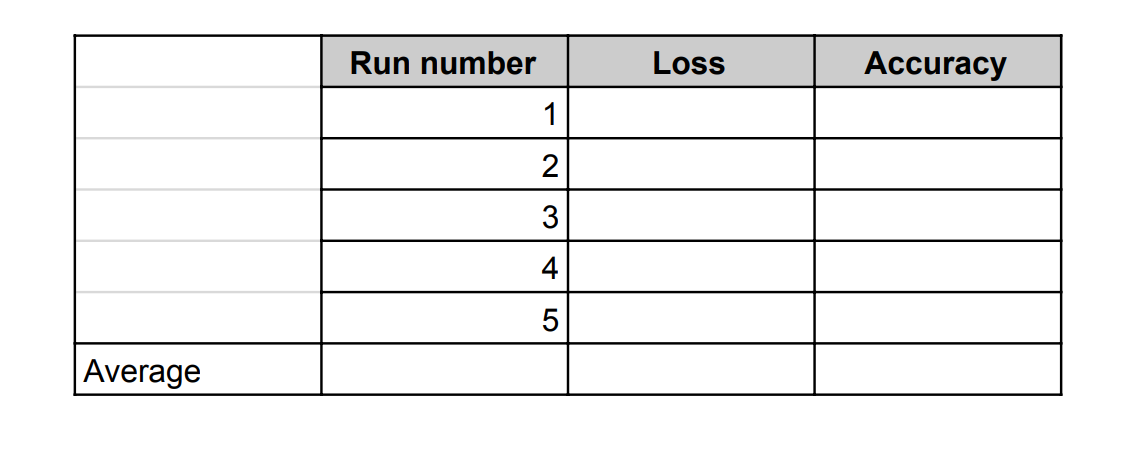
\includegraphics[scale=0.22]{figures/results.png}
    \caption{Results of five runs of the Edge-based algorithm}
    \label{fig:edge_based_met_results}
\end{figure}



Figure \ref{fig:edge_based_met_results} shows the Accuracy resp. Loss learning curve for the Edge-based method. The x-axis represents the number of iterations of the algorithm and the y-axis denotes the accuracy resp. loss.

Figure \ref{fig:missclassifications} shows an example of all  miss-classifications for one sequence. For simplicity, we only display one image frame for each sequence. On the left-hand side, we see the original image. The images on the right-hand side are then all representants of sequences wrongly classified as being of the left identity.

\begin{figure}[h!]
    \centering
    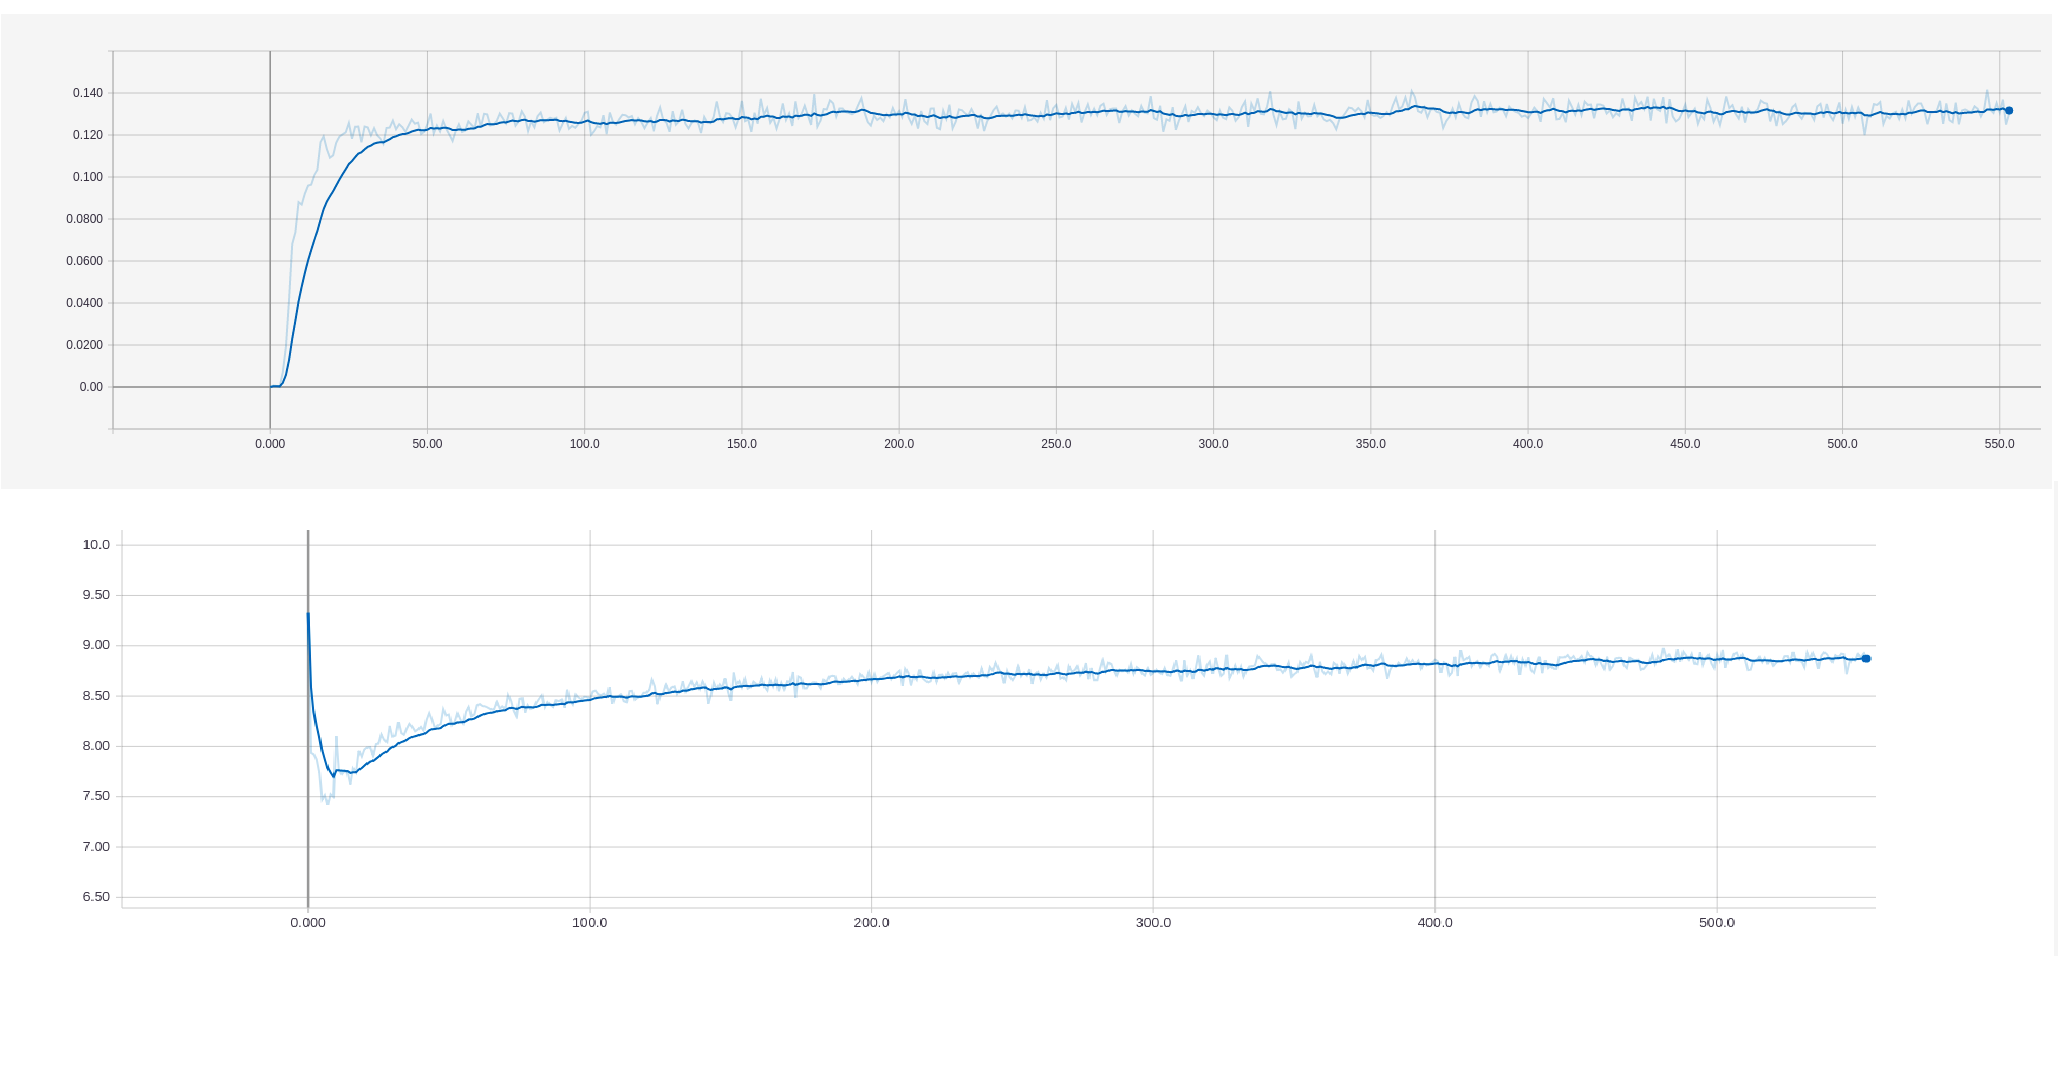
\includegraphics[scale=0.18]{figures/learning_curve.png}
    \caption{Accuracy and loss learning curves}
    \label{fig:edge_based_learning_curve_accuracy}
\end{figure}

\begin{figure}[h!]
    \centering
    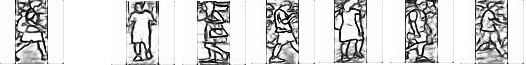
\includegraphics[scale=0.7]{figures/missclassifications.png}
    \caption{Typical miss-classifications}
    \label{fig:missclassifications}
\end{figure}

\subsubsection{Skeleton-based method}

The following table provides the results of the five independent runs of the Skeleton-based algorithm.

\begin{figure}[h!]
    \centering
    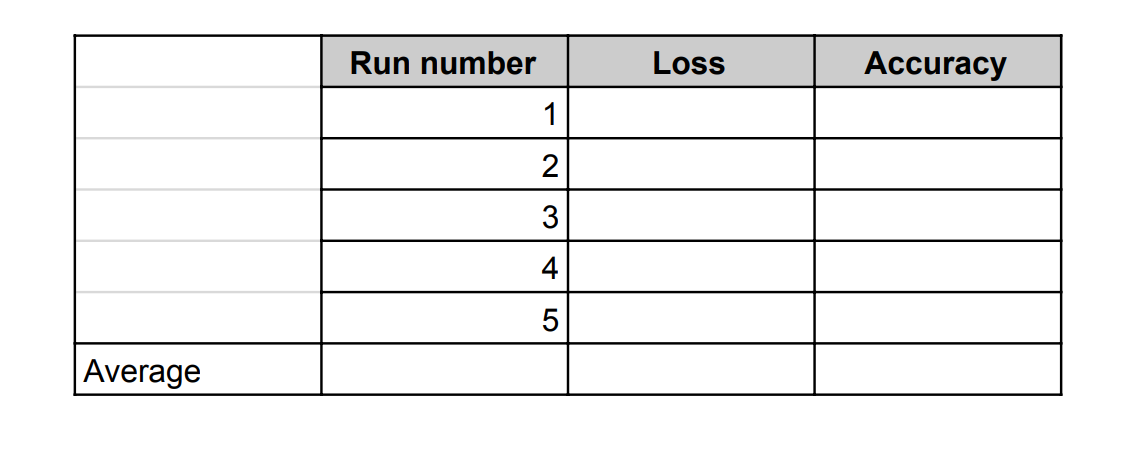
\includegraphics[scale=0.22]{figures/results.png}
    \caption{Results of five runs of the Edge-based algorithm}
    \label{fig:skeleton_based_met_results}
\end{figure}

\subsubsection{Combined method}

The following table provides the results of the five independent runs of the Edge-based algorithm.

\begin{figure}[h!]
    \centering
    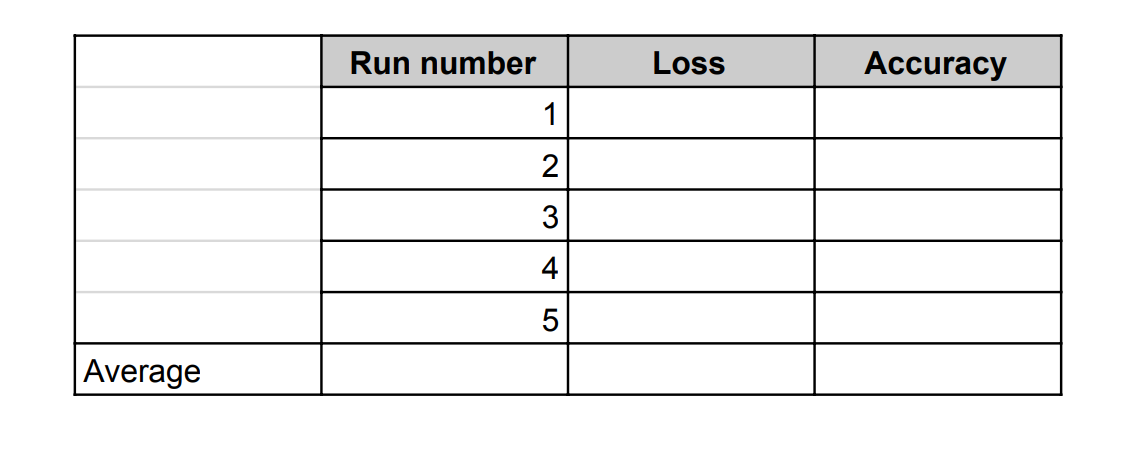
\includegraphics[scale=0.22]{figures/results.png}
    \caption{Results of five runs of the Edge-based algorithm}
    \label{fig:combined_met_results}
\end{figure}

Figures \ref{fig:combined_met_results} shows the Accuracy resp. Loss learning curve for the Combined method. The x-axis represents the number of iterations of the algorithm and the y-axis denotes the accuracy resp. loss.

\begin{figure}[h!]
    \centering
    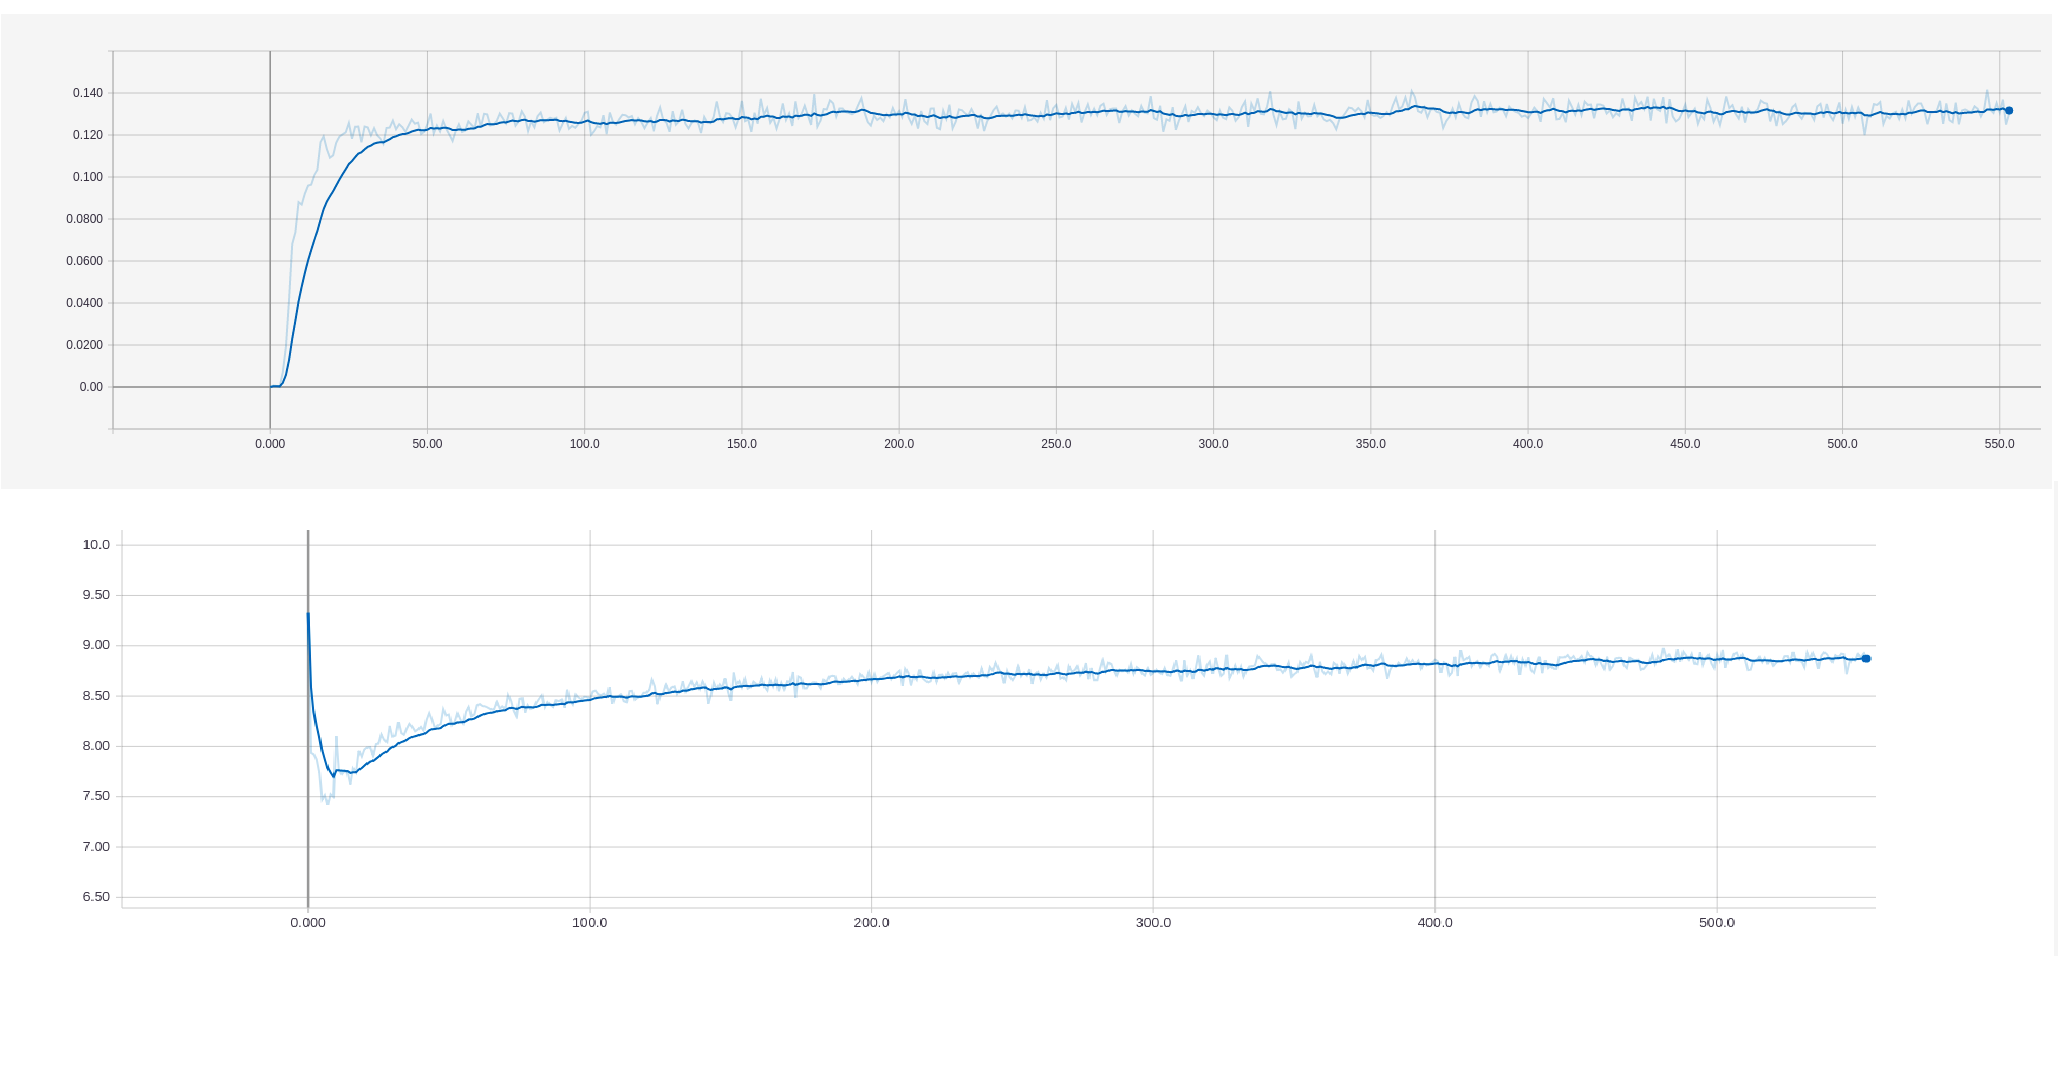
\includegraphics[scale=0.18]{figures/learning_curve.png}
    \caption{Accuracy and loss learning curves}
    \label{fig:edge_based_learning_curve_accuracy}
\end{figure}